\newpage
\section{Утилита для исследования сети и сканер портов Nmap}

\subsection{Цель работы}

Изучение работы программы Nmap на примере локальной домашней сети и сети из виртуальных машин с Kali Linux и Metasploitable2.

\subsection{Ход работы}

Эта часть работы выполняется в домашней сети 192.168.124.0/24, построенной на технологиях Fast Ethernet (IEEE 802.3u) и WiFi (IEEE 802.11n).

\subsubsection{Определение набора и версии сервисов запущенных на компьютере в диапазоне адресов}

\paragraph{Провести поиск активных хостов} Для сканирования сети будет использована команда:
\begin{Verbatim}[frame=single]
nmap -sn 192.168.124.3-255
\end{Verbatim}

Сочетание ключей s и n приводит к быстрому сканированию (т.е. без сканирования портов). Иногда это называют "ping scan" (и в старых версиях для этого использовалось "-sP"). Цель задана диапазоном IP адресов, из которого исключен роутер, и машины, с которой проводилось сканирование.

Результат сканирования:
\begin{Verbatim}[frame=single]
$ nmap -sn 192.168.124.3-255

Starting Nmap 6.40 ( http://nmap.org ) at 2015-05-18 01:01 MSK
Nmap scan report for 192.168.124.4
Host is up (0.020s latency).
Nmap scan report for 192.168.124.100
Host is up (0.00030s latency).
Nmap scan report for 192.168.124.195
Host is up (0.034s latency).
Nmap scan report for 192.168.124.239
Host is up (0.042s latency).
Nmap scan report for 192.168.124.249
Host is up (0.038s latency).
Nmap done: 253 IP addresses (5 hosts up) scanned in 2.43 seconds
\end{Verbatim}

\paragraph{Определить открытые порты}

Определим состояние 10 наиболее популярных портах на хостах из того же диапазона (стоит отметить, что хостов стало меньше)

\begin{Verbatim}[frame=single]
$ nmap --top-ports 10 192.168.124.3-255

Starting Nmap 6.40 ( http://nmap.org ) at 2015-05-18 01:26 MSK
Nmap scan report for 192.168.124.4
Host is up (0.0057s latency).
PORT     STATE  SERVICE
21/tcp   closed ftp
22/tcp   open   ssh
23/tcp   closed telnet
25/tcp   closed smtp
80/tcp   closed http
110/tcp  closed pop3
139/tcp  closed netbios-ssn
443/tcp  closed https
445/tcp  closed microsoft-ds
3389/tcp closed ms-wbt-server

Nmap scan report for 192.168.124.100
Host is up (0.00026s latency).
PORT     STATE  SERVICE
21/tcp   closed ftp
22/tcp   open   ssh
23/tcp   closed telnet
25/tcp   closed smtp
80/tcp   closed http
110/tcp  closed pop3
139/tcp  open   netbios-ssn
443/tcp  closed https
445/tcp  open   microsoft-ds
3389/tcp closed ms-wbt-server

Nmap scan report for 192.168.124.244
Host is up (0.017s latency).
PORT     STATE  SERVICE
21/tcp   closed ftp
22/tcp   closed ssh
23/tcp   closed telnet
25/tcp   closed smtp
80/tcp   closed http
110/tcp  closed pop3
139/tcp  closed netbios-ssn
443/tcp  closed https
445/tcp  closed microsoft-ds
3389/tcp closed ms-wbt-server

Nmap scan report for 192.168.124.249
Host is up (0.035s latency).
PORT     STATE  SERVICE
21/tcp   closed ftp
22/tcp   closed ssh
23/tcp   closed telnet
25/tcp   closed smtp
80/tcp   closed http
110/tcp  closed pop3
139/tcp  closed netbios-ssn
443/tcp  closed https
445/tcp  closed microsoft-ds
3389/tcp closed ms-wbt-server

Nmap done: 253 IP addresses (4 hosts up) scanned in 2.79 seconds
\end{Verbatim}

\paragraph{Определить версии сервисов} Дополнение команды ключом V приведет к определению версий (где это возможно).

\begin{Verbatim}[frame=single]
$ nmap -sV 192.168.124.3-255

Starting Nmap 6.40 ( http://nmap.org ) at 2015-05-18 01:34 MSK
Nmap scan report for 192.168.124.4
Host is up (0.029s latency).
Not shown: 999 closed ports
PORT   STATE SERVICE VERSION
22/tcp open  ssh     OpenSSH 6.8 (protocol 2.0)

Nmap scan report for 192.168.124.100
Host is up (0.00018s latency).
Not shown: 997 closed ports
PORT    STATE SERVICE     VERSION
22/tcp  open  ssh         (protocol 2.0)
139/tcp open  netbios-ssn Samba smbd 3.X (workgroup: IDEAPAD)
445/tcp open  netbios-ssn Samba smbd 3.X (workgroup: IDEAPAD)
1 service unrecognized despite returning data. If you know the
service/version, please submit the following fingerprint at
http://www.insecure.org/cgi-bin/servicefp-submit.cgi :
SF-Port22-TCP:V=6.40%I=7%D=5/18%Time=55591797%P=x86_64-pc-linux-gnu%r(NULL
SF:,29,"SSH-2\.0-OpenSSH_6\.6\.1p1\x20Ubuntu-2ubuntu2\r\n");

Nmap scan report for 192.168.124.244
Host is up (0.0080s latency).
All 1000 scanned ports on 192.168.124.244 are closed

Nmap scan report for 192.168.124.249
Host is up (0.0041s latency).
Not shown: 999 closed ports
PORT      STATE SERVICE    VERSION
62078/tcp open  tcpwrapped

Service detection performed. Please report any incorrect results
at http://nmap.org/submit/ .
Nmap done: 253 IP addresses (4 hosts up) scanned in 54.77 seconds
\end{Verbatim}

\paragraph{Изучить файлы nmap-services, nmap-os-db, nmap-service-probes}

Служебный файл \textbf{nmap-services} представляет из себя базу данных портов и протоколов (отрывок файла приведён в листинге 1). Каждая запись имеет число, определяющее вероятность того, что порт может быть открыт.

Большинство строк имеют комментарии, которые Nmap игнорирует, но пользователь может использовать GREP для получения информации о том или ином номере порта. Этот файл был изначально построен на базе список IANA, в котором сервисам распределялись порты (\url{http://www.iana.org/assignments/port-numbers}), но IANA не отслеживает порты троянов, червей и т.п., что является важным для многих пользователей Nmap.

\lstinputlisting[firstline=23,lastline=43,firstnumber=23,language={},caption={Отрывок файла nmap-services}]{res/nmap-services}

Файл \textbf{nmap-os-db} содержит сотни примеров того, как различные операционные системы ведут себя в различных ситуациях, создаваемых Nmap (листинг 2). Этот файл разделен на блоки, известные как отпечатки пальцев (fingerprints) и с каждым отпечатком соотносится имя операционной системы и её общая классификация

\lstinputlisting[firstline=21581,lastline=21597,firstnumber=21581,language={},caption={Отрывок файла nmap-os-db}]{res/nmap-os-db}

Файл \textbf{nmap-service-probes} содержит описания различных ситуация и ответного поведения сервиса (листинг 3). Это необходимо чтобы определить, какая программа прослушивает порт.

\lstinputlisting[firstline=11087,lastline=11116,firstnumber=11087,language={},caption={Отрывок файла nmap-service-probes}]{res/nmap-service-probes}

\paragraph{Добавить новую сигнатуру службы в файл nmap-service-probes} (для этого создать минимальный tcp server, добиться, чтобы при сканировании nmap указывал для него название и версию)

Исходный код простого TCP-сервера приведён в листинге 4.

\lstinputlisting[language=C++, caption={Пример простого TCP-сервера}]{../../Programming/main.c}

Простой запуск этого сервера можно обнаружить при помощи Nmap, но Nmap пока не знает, с чем имеет дело.

\begin{Verbatim}[frame=single]
$ nmap -sV -p 2404 192.168.124.4

Starting Nmap 6.40 ( http://nmap.org ) at 2015-05-18 03:42 MSK
Nmap scan report for 192.168.124.4
Host is up (0.0038s latency).
PORT     STATE SERVICE VERSION
2404/tcp open  echo

Service detection performed.
Please report any incorrect results at http://nmap.org/submit/ .
Nmap done: 1 IP address (1 host up) scanned in 41.28 seconds
\end{Verbatim}

Надо отметить, что основная идея определена верно - это действительно эхо-сервис. Но никаких данных о версии у нас нет. Теперь добавим описание сервиса в файл nmap-service-probes
\begin{Verbatim}[frame=single]
$ tail -n 7 /usr/share/nmap/nmap-service-probes
##############################NEXT PROBE##############################
# Simple TSP server.
Probe TCP simple-tcp-server-ver q|version\r\n|
rarity 9
ports 2404

match stcps m|^1\.0\.0$| p/Simple TCP Server/ v/1.0.0-3/
\end{Verbatim}

И снова проведём сканирование

\begin{Verbatim}[frame=single]
$ nmap -sV -p 2404 192.168.124.4
Starting Nmap 6.40 ( http://nmap.org ) at 2015-05-18 03:44 MSK
Nmap scan report for 192.168.124.4
Host is up (0.0035s latency).
PORT     STATE SERVICE VERSION
2404/tcp open  stcps   Simple TCP Server 1.0.0-3

Service detection performed. 
Please report any incorrect results at http://nmap.org/submit/ .
Nmap done: 1 IP address (1 host up) scanned in 6.21 seconds
\end{Verbatim}

\paragraph{Сохранить вывод утилиты в формате xml}

Вызов команды имеет следующий вид
\begin{Verbatim}[frame=single]
nmap -sV -p 2404 -oX - scanme.nmap.org 192.168.124.4
\end{Verbatim}

Результат представляет собой XML-файл
\begin{Verbatim}[frame=single]
<?xml version="1.0"?>
<?xml-stylesheet href="file:///usr/bin/../share/nmap/nmap.xsl"
                                                            type="text/xsl"?>
<!-- Nmap 6.40 scan initiated Mon May 18 03:47:51 2015
                 as: nmap -sV -p 2404 -oX - scanme.nmap.org 192.168.124.4 -->
<nmaprun scanner="nmap" args="nmap -sV -p 2404 -oX - scanme.nmap.org
              192.168.124.4" start="1431910071" startstr="Mon May 18 03:47:51
              2015" version="6.40" xmloutputversion="1.04">
<scaninfo type="connect" protocol="tcp" numservices="1" services="2404"/>
<verbose level="0"/>
<debugging level="0"/>
<host starttime="1431910071" endtime="1431910079"><status state="up"
                                       reason="conn-refused" reason_ttl="0"/>
<address addr="192.168.124.4" addrtype="ipv4"/>
<hostnames>
</hostnames>
<ports><port protocol="tcp" portid="2404"><state state="open"
              reason="syn-ack" reason_ttl="0"/><service name="stcps" product=
              "Simple TCP Server" version="1.0.0-3" method="probed" conf="10"/>
              </port>
</ports>
<times srtt="4122" rttvar="2991" to="100000"/>
</host>
<runstats><finished time="1431910079" timestr="Mon May 18 03:47:59 2015"
               elapsed="7.40" summary="Nmap done at Mon May 18 03:47:59 2015;
               2 IP addresses (1 host up) scanned in 7.40 seconds"
               exit="success"/><hosts up="1" down="1" total="2"/>
</runstats>
</nmaprun>
\end{Verbatim}

\paragraph{Исследовать различные этапы и режимы работы nmap с использованием утилиты Wireshark}

На рисунке 1 показано сканирование порта 2404 (по совпадению, он имеет имя iec-104). Видно, что в пакете передаётся запрос "version". А на рисунке 2 опрос 10 наиболее популярных портов.

\begin{figure}[h!]
\centering
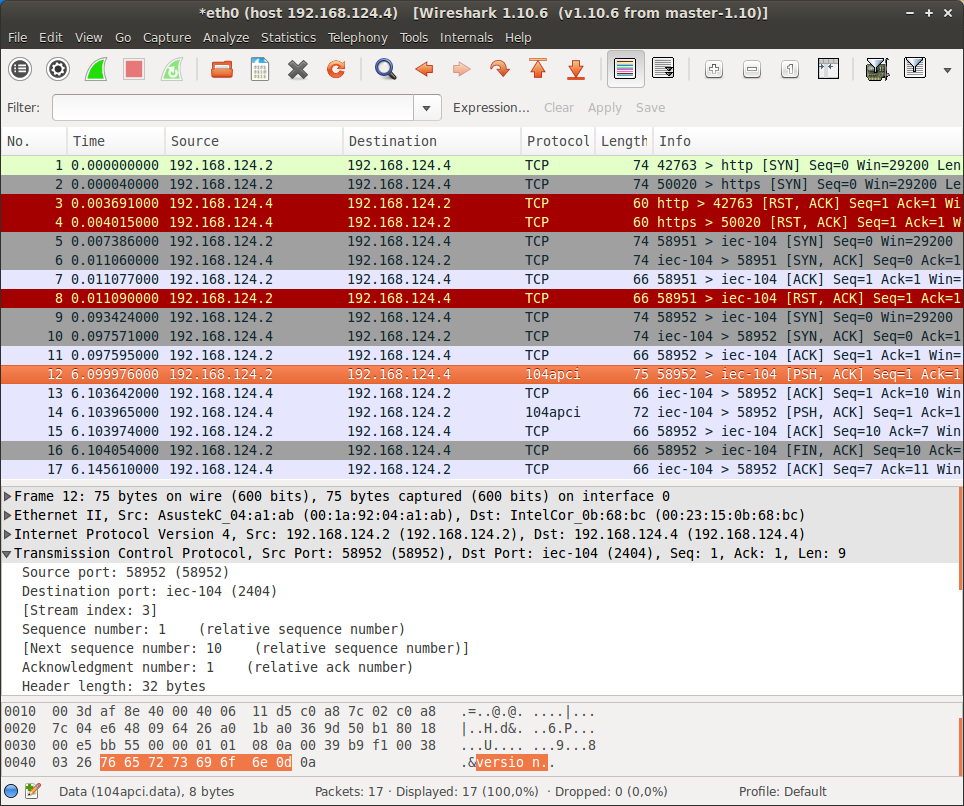
\includegraphics[scale=0.45]{res/pic01}
\caption{Определение сервиса на порт 2040}
\end{figure}

\begin{figure}[h!]
\centering
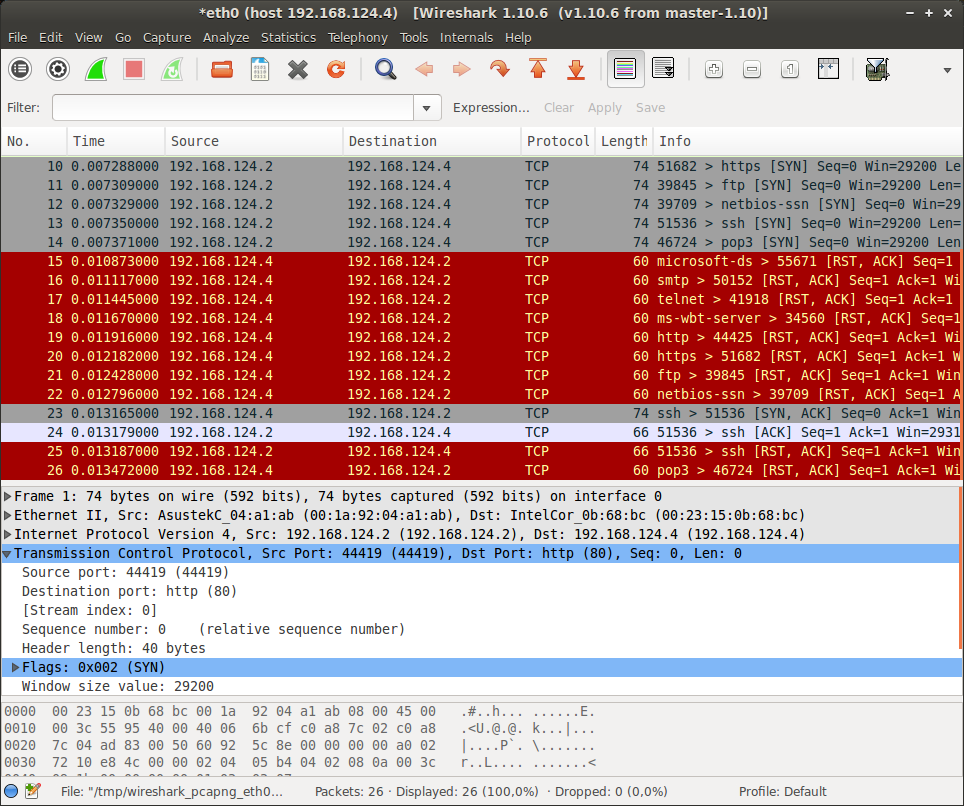
\includegraphics[scale=0.45]{res/pic02}
\caption{Опрос 10 наиболее популярных портов}
\end{figure}

\newpage
\subsubsection{Просканировать виртуальную машину Metasploitable2 используя db\_nmap из состава metasploit\-framework}

% applications > kali linux > system services > metasploit > start

% applications > kali linux > top 10 security tools > metasploit framework

% msfconsole

Стоит отметить, что Metasploitable2 достаточно прожорлив в плане ресурсов, особенно по части оперативной памяти. Это является результатом большого количества запущенных сервисов.

\begin{Verbatim}[frame=single]
msf > db_nmap -v -sV 192.168.124.211
[*] Nmap: Starting Nmap 6.47 ( http://nmap.org ) at 2015-05-18 21:05 UTC
[*] Nmap: NSE: Loaded 29 scripts for scanning.
[*] Nmap: Initiating ARP Ping Scan at 21:05
[*] Nmap: Scanning 192.168.124.211 [1 port]
[*] Nmap: Completed ARP Ping Scan at 21:05, 0.05s elapsed (1 total hosts)
[*] Nmap: Initiating Parallel DNS resolution of 1 host. at 21:05
[*] Nmap: Completed Parallel DNS resolution of 1 host. at 21:05, 0.01s
                                                                      elapsed
[*] Nmap: Initiating SYN Stealth Scan at 21:05
[*] Nmap: Scanning 192.168.124.211 [1000 ports]
[*] Nmap: Discovered open port 22/tcp on 192.168.124.211
[*] Nmap: Discovered open port 5900/tcp on 192.168.124.211
[*] Nmap: Discovered open port 80/tcp on 192.168.124.211
[*] Nmap: Discovered open port 53/tcp on 192.168.124.211
[*] Nmap: Discovered open port 21/tcp on 192.168.124.211
[*] Nmap: Discovered open port 3306/tcp on 192.168.124.211
[*] Nmap: Discovered open port 445/tcp on 192.168.124.211
[*] Nmap: Discovered open port 23/tcp on 192.168.124.211
[*] Nmap: Discovered open port 25/tcp on 192.168.124.211
[*] Nmap: Discovered open port 111/tcp on 192.168.124.211
[*] Nmap: Discovered open port 139/tcp on 192.168.124.211
[*] Nmap: Discovered open port 2049/tcp on 192.168.124.211
[*] Nmap: Discovered open port 512/tcp on 192.168.124.211
[*] Nmap: Discovered open port 8180/tcp on 192.168.124.211
[*] Nmap: Discovered open port 6000/tcp on 192.168.124.211
[*] Nmap: Discovered open port 5432/tcp on 192.168.124.211
[*] Nmap: Discovered open port 1524/tcp on 192.168.124.211
[*] Nmap: Discovered open port 1099/tcp on 192.168.124.211
[*] Nmap: Discovered open port 6667/tcp on 192.168.124.211
[*] Nmap: Discovered open port 514/tcp on 192.168.124.211
[*] Nmap: Discovered open port 2121/tcp on 192.168.124.211
[*] Nmap: Discovered open port 8009/tcp on 192.168.124.211
[*] Nmap: Discovered open port 513/tcp on 192.168.124.211
[*] Nmap: Completed SYN Stealth Scan at 21:05, 0.55s elapsed (1000 total
                                                                       ports)
[*] Nmap: Initiating Service scan at 21:05
[*] Nmap: Scanning 23 services on 192.168.124.211
[*] Nmap: Completed Service scan at 21:05, 11.76s elapsed (23 services on 1
                                                                        host)
[*] Nmap: NSE: Script scanning 192.168.124.211.
[*] Nmap: Initiating NSE at 21:05
[*] Nmap: Completed NSE at 21:05, 0.16s elapsed
[*] Nmap: Nmap scan report for 192.168.124.211
[*] Nmap: Host is up (0.00030s latency).
[*] Nmap: Not shown: 977 closed ports
[*] Nmap: PORT     STATE SERVICE     VERSION
[*] Nmap: 21/tcp   open  ftp         vsftpd 2.3.4
[*] Nmap: 22/tcp   open  ssh         OpenSSH 4.7p1 Debian 8ubuntu1 (protocol
                                                                         2.0)
[*] Nmap: 23/tcp   open  telnet      Linux telnetd
[*] Nmap: 25/tcp   open  smtp        Postfix smtpd
[*] Nmap: 53/tcp   open  domain      ISC BIND 9.4.2
[*] Nmap: 80/tcp   open  http        Apache httpd 2.2.8 ((Ubuntu) DAV/2)
[*] Nmap: 111/tcp  open  rpcbind     2 (RPC #100000)
[*] Nmap: 139/tcp  open  netbios-ssn Samba smbd 3.X (workgroup: WORKGROUP)
[*] Nmap: 445/tcp  open  netbios-ssn Samba smbd 3.X (workgroup: WORKGROUP)
[*] Nmap: 512/tcp  open  exec        netkit-rsh rexecd
[*] Nmap: 513/tcp  open  login
[*] Nmap: 514/tcp  open  tcpwrapped
[*] Nmap: 1099/tcp open  rmiregistry GNU Classpath grmiregistry
[*] Nmap: 1524/tcp open  shell       Metasploitable root shell
[*] Nmap: 2049/tcp open  nfs         2-4 (RPC #100003)
[*] Nmap: 2121/tcp open  ftp         ProFTPD 1.3.1
[*] Nmap: 3306/tcp open  mysql       MySQL 5.0.51a-3ubuntu5
[*] Nmap: 5432/tcp open  postgresql  PostgreSQL DB 8.3.0 - 8.3.7
[*] Nmap: 5900/tcp open  vnc         VNC (protocol 3.3)
[*] Nmap: 6000/tcp open  X11         (access denied)
[*] Nmap: 6667/tcp open  irc         Unreal ircd
[*] Nmap: 8009/tcp open  ajp13       Apache Jserv (Protocol v1.3)
[*] Nmap: 8180/tcp open  http        Apache Tomcat/Coyote JSP engine 1.1
[*] Nmap: MAC Address: 08:00:27:6E:3D:DB (Cadmus Computer Systems)
[*] Nmap: Service Info: Hosts:  metasploitable.localdomain, localhost, 
     irc.Metasploitable.LAN; OSs: Unix, Linux; CPE: cpe:/o:linux:linux_kernel
[*] Nmap: Read data files from: /usr/bin/../share/nmap
[*] Nmap: Service detection performed. Please report any incorrect results at
                                                    http://nmap.org/submit/ .
[*] Nmap: Nmap done: 1 IP address (1 host up) scanned in 14.14 seconds
[*] Nmap: Raw packets sent: 1001 (44.028KB) | Rcvd: 1001 (40.120KB)
msf > 
\end{Verbatim}

\subsubsection{Выбрать пять записей из файла nmap-service-probes и описать их работу.}

Рассмотрим подробнее листинг 3. Он описывает поведение различных сервисов, работающих с SIP-протоколом.

Строка \textbf{11087} не никакой смысловой нагрузки не несёт. Она отделяет один набор правил от другого.

В строке \textbf{11088} представлена директива probe. Она используется для указания того, какие данные отправлять в процессе определения службы. Синтаксис команды имеет следующий вид:
\begin{Verbatim}[frame=single]
probe <protocol> <probename> <probesendstring> 
\end{Verbatim}
где
\begin{itemize}
  \item Protocol — тип протокола (может быть или TCP или UDP).
  \item Probename — название теста. Используется в отпечатке службы для указания, на какой тест был получен ответ. Название может быть произвольным (удобным для пользователя). 
  \item Probesendstring — строка, используемая для тестового запроса. Должна начинаться символами "q|" и заканчиваться символом "|". Между ограничителями находится непосредственно сама строка, передаваемая в качестве теста. Эта строка имеет формат, аналогичный строкам языков C или Perl, и может содержать стандартные escape-последовательности.
\end{itemize}

В рассматриваемой строке тип протокола UDP, название теста SIPOptions, а запрос имеет следующий вид:
\begin{Verbatim}[frame=single]
OPTIONS sip:nm SIP/2.0
Via: SIP/2.0/TCP nm;branch=foo
From: <sip:nm@nm>;tag=root
To: <sip:nm2@nm2>
Call-ID: 50000
CSeq: 42 OPTIONS
Max-Forwards: 70
Content-Length: 0
Contact: <sip:nm@nm>
Accept: application/sdp

\end{Verbatim}

В строке \textbf{11089} параметру rarity присвоено значение 6. Чем выше его значение (максимум 9), тем меньше шансов ожидать результатов от этого теста.

Строка \textbf{11090} указывает на номер порта, которому будут отправлены данные из директивы probe. В нашем случае используется стандартный порт 5060, но  в общем случае портов может быть несколько (тогда их перечисляют через запятую) или требуется установить шифрованное соединение по SSL (тогда вместо ports используется директива sslports).

Строку \textbf{11091} можно пропустить. т.к. она содержит комментарий, а вот строка \textbf{11092} содержит полезный материал - указывает сколько времени (в миллисекундах) необходимо ждать ответ, прежде чем прекратить тест службы. Иногда VoIP устройства отвечают с задержкой, и для этого используется директива totalwaitms. В нашем случае время ожидания составит 7500 мс.

Далее стоит рассмотреть группу строк с \textbf{11094} по \textbf{11112}. Директива match указывает nmap на то, как точно определить службу, используя полученный ответ на запрос, отправленный предыдущей директивой probe. Эта директива используется в случае, когда полученный ответ полностью совпадает с шаблоном. При этом тестирование порта считается законченным, а при помощи дополнительных спецификаторов nmap строит отчет о названии приложения, номере версии и дополнительной информации, полученной в ходе проверки. Синтаксис директивы match:
\begin{Verbatim}[frame=single]
match <service> <pattern> <productname> <version> <device> <h???> <info> <OS>
\end{Verbatim}
где
\begin{itemize}
  \item service -- название службы, для которой приведен шаблон (например: ssh, smtp, http или SNMP). 
  \item pattern -- шаблон (литерал m указывает на начало строки, сам шаблон находится между символами прямой "|" или правый "/" слэш), с которым должен совпадать полученный ответ. Формат шаблона аналогичен принятому в языке Perl
  \item productname -- поле (указывается символом "p") указывает название производителя или имя службы.
  \item version -- поле (указывается символом "v") указывает версию опознано службы, устройства, ОС или программы. Оно может содержать как числовой формат, так и несколько слов (иногда указывается что версия не известна). Может отсутствовать.
  \item Device -- поле (указывается символом "d") указывает распознанное устройство. Может отсутствовать.
  \item h??? -- назначение флага не определено!
  \item info -- поле (указывается символом "i") указывает дополнительную полезную информацию, которая может пригодиться на этапе сканирования (например, номер протокола сервера ssh). Может отсутствовать.
  \item OS -- поле (указывается символом "o") указывает операционную систему, при условии, что она распознана. Может отсутствовать.
\end{itemize}

Таким образом, если в ответ на запрос из директивы probe придёт примерно такой ответ
\begin{Verbatim}[frame=single]
SIP/2.0 200 OK
User-Agent: SAGEM / 3202.3 / 2601EC
\end{Verbatim}
то это устройство Sagem ADSL router из строки 11097.

Две строки \textbf{11113} по \textbf{11114} содержат директиву softmatch. Директива softmatch имеет аналогичный формат директиве match. Основное отличие заключается в том, что после совпадения принятого ответа с одним из шаблонов softmatch, тестирование будет продолжено с использованием только тех тестов, которые относятся к определенной шаблоном службе. Тестирование порта будет идти до тех пор, пока не будет найдено строгое соответствие (match) или не закончатся все тесты для данной службы.

\subsubsection{Выбрать один скрипт из состава Nmap и описать его работу.}

Рассмотрим маленький скрипт smtp-strangeport.nse ил листинга 5.

\lstinputlisting[language={},caption={скрипт smtp-strangeport.nse}]{res/smtp-strangeport.nse}

В первой строчке даёт описание назначение этого модуля - он проверяет наличие SMTP-шлюза, работающего на нестандартном порту. Такая проверка может быть актуальна после взлома, чтобы удостовериться что с машины не происходит рассылка спама.

В 13-й строке указан автор, в 15-й -- тип лицензии (совпадает с лицензией nmap).

В строке 17 определены категории скрипта. Всего существует порядка 10 категорий. Категория malware говорит что назначение скрипта состоит в проверке исследуемой системы на следы заражения вредоносной программы (malware), а категория safe - что скрипт безопасен, и его работа не приведёт к некорректной работе или остановке какого-либо сервиса.

Основная функция представлена в строке 19. Она возвращает значение TRUE, если обнаружит открытый TCP-сокет с SMTP сервисом с не стандартным номером (стандартные номера это 25, 465 и 587).

Эта функция вызывается из точки входа программы, в строке 26.

\subsection{Выводы}

Инструмент nmap является мощным средством для исследования новой сети или изучения последствий внешнего проникновения. Встроенный механизм скриптов (Nmap Scripting Engine - NSE) позволяет расширить его функциональность для дополнительных задач. Сохранение результатов в XML упрощает дальнейший анализ результатов и позволяет автоматизировать процесс наблюдения за сетью.
